% =============================================================================
% The step_7 architecture — an explanatory packet for the Solanus archival tool.
%
% Build (keeps ALL aux/intermediary files in a build/ subfolder, so only
% architecture.tex and architecture.pdf sit in this directory):
%
%     latexmk -pdf -outdir=build architecture.tex
%
% then (optionally) copy the PDF up next to the source:
%     cp build/architecture.pdf .
%
% Nothing exotic is required; the TikZ figures are self-contained.
% =============================================================================
\documentclass[11pt]{article}
\usepackage{lmodern}
\usepackage[T1]{fontenc}

% --- Packages ---------------------------------------------------------------
\usepackage[margin=1in]{geometry}
\usepackage{amsmath,amssymb}
\usepackage{microtype}
% microtype's font EXPANSION needs scalable Type1 fonts in the pdftex map; some minimal TeX
% installs ship the listings/typewriter fonts as non-scalable, which makes expansion fatal. We keep
% all of microtype's other benefits (character protrusion, smarter spacing) and switch off only
% expansion, so the doc compiles on a bare install AND a full one. Drop this line on a full TeX Live.
\microtypesetup{expansion=false}
\usepackage{enumitem}
\usepackage{xcolor}
\usepackage{hyperref}
\usepackage{listings}
\usepackage{booktabs}
\usepackage{tikz}
\usepackage[most]{tcolorbox}
\usepackage{placeins}   % \FloatBarrier to keep figures inside their section
\usepackage{caption}
\usetikzlibrary{arrows.meta, positioning, decorations.pathreplacing,
                calc, shapes.geometric, fit, backgrounds, patterns}

\captionsetup{font=small,skip=8pt}
\setlength{\textfloatsep}{18pt plus 4pt minus 4pt}
\setlength{\intextsep}{16pt plus 4pt minus 4pt}

\hypersetup{colorlinks=true, linkcolor=blue!50!black,
            urlcolor=blue!50!black, citecolor=blue!50!black}

% --- Listings (Python / shell) ----------------------------------------------
\definecolor{codebg}{RGB}{248,248,248}
\definecolor{codekw}{RGB}{0,0,180}
\definecolor{codecmt}{RGB}{0,128,0}
\definecolor{codestr}{RGB}{170,55,0}
\lstset{
  basicstyle=\ttfamily\small,
  backgroundcolor=\color{codebg},
  keywordstyle=\color{codekw}\bfseries,
  commentstyle=\color{codecmt}\itshape,
  stringstyle=\color{codestr},
  showstringspaces=false,
  language=Python,
  breaklines=true,
  columns=fullflexible,
  frame=single,
  framesep=4pt,
  rulecolor=\color{black!20},
}

% --- Coloured callout boxes (cf. the intuitive-writeup example) -------------
\newtcolorbox{tldr}[1][]{
  colback=blue!5, colframe=blue!50!black, fonttitle=\bfseries,
  title={#1}, sharp corners, boxrule=0.6pt}
\newtcolorbox{keybox}[1][]{
  colback=green!5, colframe=green!45!black, fonttitle=\bfseries,
  title={#1}, sharp corners, boxrule=0.6pt}
\newtcolorbox{caveatbox}[1][]{
  colback=yellow!10, colframe=orange!70!black, fonttitle=\bfseries,
  title={#1}, sharp corners, boxrule=0.6pt}

% --- Convenience macros -----------------------------------------------------
\newcommand{\code}[1]{\texttt{#1}}
\newcommand{\stage}[1]{\textbf{\texttt{#1}}}

\title{\bfseries The \texttt{step\_7} Architecture\\[2pt]
\large How the Solanus Casey archival tool is built}
\author{David Falk \\ Solanus Project Pipeline}
\date{}

\begin{document}
\maketitle
\tableofcontents
\bigskip

%==============================================================================
\section{TL;DR}
%==============================================================================

\begin{tldr}[The whole machine in six sentences]
\begin{itemize}[leftmargin=1.2em, itemsep=3pt]
  \item \textbf{One DAG, re-run only what changed.} Every unit of work is a content-hashed
        \code{Stage}; a stage is \emph{stale} if its inputs, its code, the config, or any upstream
        stage changed, and \code{run()} re-executes the stale stages \emph{and everything
        downstream}.
  \item \textbf{Three swappable model axes.} Generation \textbf{LLM}, \textbf{embedding} space, and
        \textbf{reranker} are config variables behind thin adapters --- swapping one is an edit to a
        dict, never a rewrite of the code that uses it.
  \item \textbf{Every model call is cost-logged, always.} Nothing calls a provider directly; one
        funnel (\code{lib/costlog.py}) records every billed call, so the dollar ledger is complete
        and the free path stays free.
  \item \textbf{Provenance is first-class.} Every chunk, fact, and answer cites
        \code{doc\_id\,+\,rid\,+\,page\,+\,vertices} --- the exact polygon on the exact scanned page.
  \item \textbf{Non-destructive, always.} Stages only write new artifacts; the runner never deletes;
        \code{step\_6/} source data is read-only.
  \item \textbf{Tiered, so you choose your altitude.} Tier~0 solid RAG $\rightarrow$ Tier~1
        structural truth $\rightarrow$ Tier~2 knowledge graph $\rightarrow$ Tier~3 multimodal
        $\rightarrow$ Tier~4 scholarly platform.
\end{itemize}
\end{tldr}

%==============================================================================
\section{Key points (the five design commitments)}
%==============================================================================

Everything below is a consequence of five commitments. They are not slogans --- each one is enforced
by a specific piece of code you can open and read.

\begin{keybox}[The five commitments]
\begin{enumerate}[leftmargin=1.4em, itemsep=2pt]
  \item \textbf{Diff-and-rerun reproducibility} --- a content-hashed stage DAG; staleness propagates.
        (\code{lib/pipeline.py})
  \item \textbf{Always log prices} --- one funnel records every billed call; the free path is free.
        (\code{lib/costlog.py})
  \item \textbf{Model-agnostic, three axes} --- LLM / embedding / reranker are config variables
        behind adapters. (\code{config.py}, \code{lib/providers/})
  \item \textbf{Provenance-first + archival standards} --- cite \code{doc\_id+rid+page+vertices};
        graph aligned to RiC-O; dates in EDTF.
  \item \textbf{Expandable} --- add a stage, an embedding space, a model, or a tool without touching
        the rest.
\end{enumerate}
\end{keybox}

%==============================================================================
\section{The corpus we start from}
%==============================================================================

Before any of the machinery makes sense, you need to see the shape of the raw material, because the
architecture is built \emph{around} that shape. \code{step\_6} hands us two read-only JSON files.

\paragraph{\code{documents.json} --- 570 letters.} Each record carries an \code{id} (e.g.\
\code{Volume\_1\_\_p001}), a \code{recipient}, a \code{date} (e.g.\ ``Aug.\ 23rd, 1896''), and --- the
useful part --- a \code{text\_by\_label} dict that \emph{already separates} the letter into labelled
fields: \code{src\_content}, \code{src\_recipient}, \code{src\_greeting}, \code{src\_date},
\code{src\_signature}, \code{archv\_date}, and so on. It also carries \code{regions[]}, where each
region has a \code{rid}, a \code{category}, the OCR \code{text}, an OCR \code{min\_conf}, and the gold
polygon \code{vertices} (pixel geometry on the page).

\paragraph{\code{notebooks.json} --- 716 notebook pages.} These are Fr.\ Solanus's running register of
favours. Each page has a \code{notebook} name (e.g.\ ``FR.\ SOLANUS, NOTEBOOK NO.\ 1.''), a
\code{pdf\_page\_number}, an archival \code{archv\_date}, and an \code{entries[]} list. Each
\emph{entry} carries its \code{rid}, its \code{text}, a \code{date} (often just ``30'' or
``Mar.\ 30''), a \code{page\_label} (literally ``Page 1 Cont.'' for spill-over pages), and
\code{linked} (degree-1 links from the gold connection graph).

Two features of this shape drive the entire design: \textbf{labelled fields you can read off for
free}, and \textbf{per-region geometry you can cite}. \code{lib/chunks.py} turns the two files into
$\sim$\textbf{9{,}342 retrieval chunks} (one per letter, one per notebook entry), each carrying its
provenance metadata so any hit can point back at the exact region it came from.

\begin{tcolorbox}[colback=gray!5, colframe=gray!50!black, sharp corners, boxrule=0.5pt,
                  title=\bfseries A concrete entry that explains why half the pipeline exists]
The notebook entry \code{doc\_1.src\_content.4} stores its date as the bare string \code{"30"} and is
\code{linked} to \code{doc\_1.src\_content.10}; the page above it is labelled \code{"Page 1 Cont."}.
On its own, that entry --- no year, half a thought, continued from somewhere else --- is almost
invisible to a search engine. The structural-truth stages (\S\ref{sec:tiers}) exist precisely to
rebuild the \emph{whole} favour, with its date, before anything tries to retrieve it.
\end{tcolorbox}

%==============================================================================
\section{The diff-and-rerun pipeline}\label{sec:pipeline}
%==============================================================================

This is the single most important idea in \code{step\_7}, so we build it up slowly.

\subsection{The intuition: a recipe that re-cooks only what changed}

Picture the whole build as a recipe where each step depends on earlier ones: chop the vegetables,
then sauté them, then simmer. If you change one early ingredient, you want \emph{only} the affected
later steps to re-cook --- not the entire meal (wasteful), and not nothing (you'd serve stale food).
That is exactly what the pipeline does, automatically, for a graph of build steps.

\subsection{A \texttt{Stage} declares four things}

Each unit of work is a \code{Stage} that names its dependencies, what it reads, and what it writes:

\begin{lstlisting}
Stage(name      = "embed_corpus",
      fn        = embed_corpus.run,           # the function that does the work
      deps      = [...],                       # upstream stage names it depends on
      inputs    = [DOCS, NB, ".../embed.py"],  # path globs it READS
      outputs   = [str(DATA / "vectors")])     # path globs it WRITES
\end{lstlisting}

\subsection{The fingerprint: four ingredients, any one of which makes a stage stale}

A stage's \textbf{fingerprint} is a SHA-256 hash over four things. The cleverness is in \emph{what}
goes into the hash --- it is chosen so that the four ways a result can become out-of-date all map to
``the hash changed.''

\begin{enumerate}[leftmargin=1.6em, itemsep=2pt]
  \item \textbf{The source code of \code{fn()}} (via \code{inspect.getsource}) --- so editing the
        stage's logic re-runs it.
  \item \textbf{The config fingerprint} (\code{config.fingerprint()}) --- so changing a model, a
        price, or the embedding matrix re-runs the stages that depend on config.
  \item \textbf{The contents of every input file} --- so refining the upstream data re-runs the stage.
  \item \textbf{The fingerprints of all upstream stages} --- so staleness \emph{cascades} downstream
        automatically.
\end{enumerate}

\begin{figure}[h]
\centering
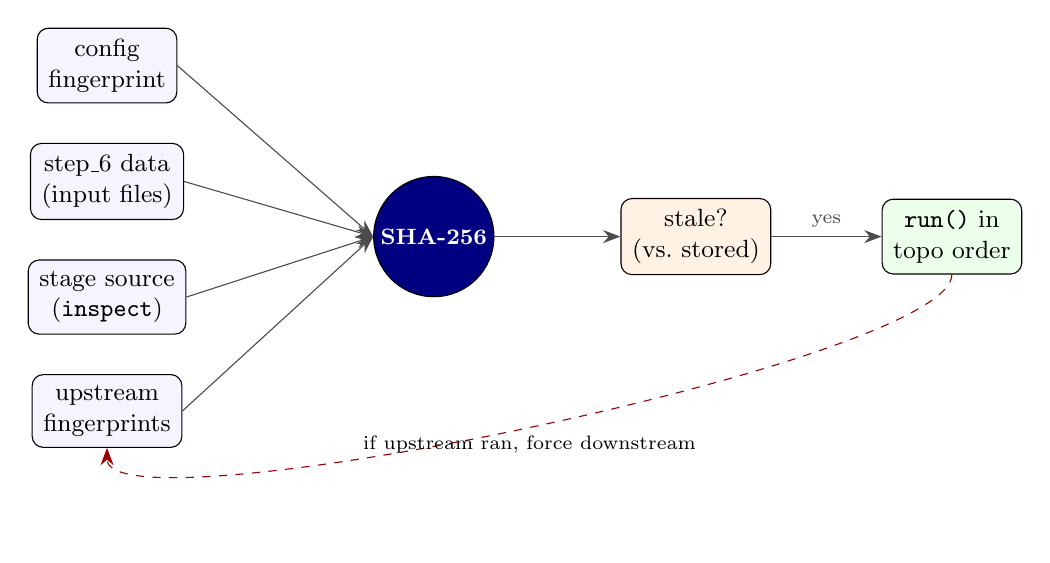
\begin{tikzpicture}[
    node distance=5mm,
    box/.style={draw, rounded corners, align=center, font=\small, inner sep=4pt, fill=blue!4},
    hash/.style={draw, circle, font=\footnotesize\bfseries, inner sep=2pt, fill=blue!50!black, text=white},
    arr/.style={-{Stealth[length=2.2mm]}, gray!60!black}]
  \node[box] (cfg)  {config\\ fingerprint};
  \node[box, below=of cfg] (data) {step\_6 data\\ (input files)};
  \node[box, below=of data] (src)  {stage source\\ (\code{inspect})};
  \node[box, below=of src]  (up)   {upstream\\ fingerprints};
  \node[hash, right=24mm of data, yshift=-7mm] (h) {SHA-256};
  \node[box, right=16mm of h, fill=orange!10] (stale) {stale?\\ (vs.\ stored)};
  \node[box, right=14mm of stale, fill=green!8] (run) {\code{run()} in\\ topo order};
  \foreach \n in {cfg,data,src,up} \draw[arr] (\n.east) -- (h.west);
  \draw[arr] (h) -- (stale);
  \draw[arr] (stale) -- node[above, font=\scriptsize]{yes} (run);
  % downstream-forcing feedback loop
  \draw[arr, dashed, red!60!black] (run.south) .. controls +(0,-1.1) and +(0,-1.1) ..
        node[below, font=\scriptsize, black]{if upstream ran, force downstream} (up.south);
\end{tikzpicture}
\caption{The fingerprint funnel. Any of the four inputs changing flips the stage to \emph{stale};
running a stage forces everything downstream of it to run too (red loop) --- which is how a fix to an
early artifact ``populates all the way up.''}
\end{figure}

\subsection{What ``stale'' means, and the one magic line}

A stage is \textbf{stale} when its fingerprint differs from the stored one (in
\code{\_pipeline\_state.json}), \emph{or} an output file is missing, \emph{or} an upstream stage
re-ran this pass. \code{status()} prints the diff first (read-only); \code{run()} executes stale
stages in topological order and --- this is the magic line --- \textbf{forces everything downstream of
anything that runs.} So if you refine the cleaned OCR text, the rerun naturally flows entities
$\rightarrow$ resolution $\rightarrow$ graph $\rightarrow$ embeddings $\rightarrow$ indexes,
``populating all the way up'' with no manual bookkeeping.

\begin{figure}[h]
\centering
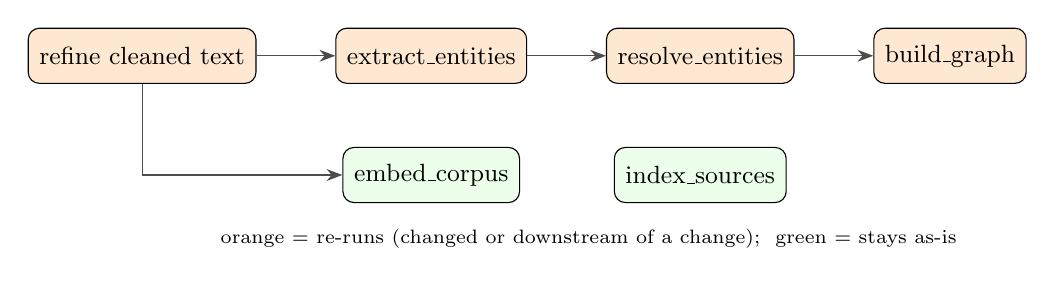
\begin{tikzpicture}[
    n/.style={draw, rounded corners, font=\small, inner sep=4pt, minimum height=7mm},
    fresh/.style={n, fill=green!8}, stale/.style={n, fill=orange!18},
    arr/.style={-{Stealth[length=2mm]}, gray!60!black}]
  \node[stale] (clean) {refine cleaned text};
  \node[stale, right=10mm of clean] (ner) {extract\_entities};
  \node[stale, right=10mm of ner]  (res) {resolve\_entities};
  \node[stale, right=10mm of res]  (kg)  {build\_graph};
  \node[fresh, below=8mm of ner]   (emb) {embed\_corpus};
  \node[fresh, below=8mm of res]   (idx) {index\_sources};
  \draw[arr] (clean) -- (ner); \draw[arr] (ner) -- (res); \draw[arr] (res) -- (kg);
  \draw[arr] (clean.south) |- (emb.west);
  \node[font=\scriptsize, align=center, below=2mm of emb, xshift=20mm]
        {orange = re-runs (changed or downstream of a change);\ \ green = stays as-is};
\end{tikzpicture}
\caption{Editing one upstream artifact (left) marks it stale and cascades to everything that depends
on it; unrelated branches stay fresh and are skipped.}
\end{figure}

\subsection{Two guardrails}

\begin{itemize}[leftmargin=1.4em, itemsep=2pt]
  \item \textbf{Non-destructive.} Stages only write \emph{new} artifacts; the runner \emph{never
        deletes}. \code{step\_6/} source data is never touched --- you can always recover.
  \item \textbf{Stdlib only.} The engine is just hashing, \code{glob}, and a JSON state file --- zero
        dependencies --- so the reproducibility backbone can never rot because a library moved.
\end{itemize}

\subsection{Driving it}

You declare the DAG and drive it from \code{run.py}:

\begin{lstlisting}[language=bash]
python run.py status            # show the diff: what's stale and WHY  (read-only)
python run.py run               # run all stale stages + everything downstream
python run.py run --only embed_corpus
python run.py run --dry         # report what WOULD run; execute nothing
python run.py graph             # print the dependency DAG
\end{lstlisting}

Nothing runs on import, and unimplemented stages raise \code{NotImplementedError} --- so the DAG is
fully \emph{inspectable} long before it is fully \emph{runnable}. That is deliberate: David runs paid
stages explicitly, when ready.

\FloatBarrier
%==============================================================================
\section{The model-agnostic three-axis design}\label{sec:axes}
%==============================================================================

A RAG system plugs a model into exactly three places. \code{step\_7} treats each as a \textbf{variable
you select}, not a dependency you hard-wire.

\begin{table}[h]
\centering\small
\begin{tabular}{@{}llll@{}}
\toprule
\textbf{Axis} & \textbf{What it does} & \textbf{Where it lives} & \textbf{Adapter} \\
\midrule
LLM & reads context, writes the cited answer, drives tool-use & \code{config.LLMS} & \code{providers/llm.py} \\
Embedding & turns text into a vector for similarity search & \code{config.EMBEDDINGS} & \code{providers/embed.py} \\
Reranker & sharp 2nd-stage judge (``retrieve 50, rerank to 5'') & \code{config.RERANKERS} & \code{providers/rerank.py} \\
\bottomrule
\end{tabular}
\caption{The three swappable axes. Each is a registry dict in \code{config.py} read through a thin
adapter; the stages and the app never import a vendor SDK.}
\end{table}

\subsection{The pattern (the same for all three)}

Internalise this once and every future model plugs in the same way: a single public function
(\code{generate} / \code{embed\_texts} / \code{rerank}) looks up \code{provider} in the config dict
and dispatches to a small per-provider implementation. Each implementation is the \emph{only} place
that imports a vendor SDK, so adding a Claude or OpenAI model is one new branch next to the Gemini
one --- the rest of the system doesn't notice.

\begin{lstlisting}
def generate(prompt, model=None, ...):
    model = model or config.DEFAULTS["llm"]
    prov  = config.LLMS.get(model, {}).get("provider", "gemini")
    if prov == "gemini":
        return _gemini(prompt, model, ...)   # the ONE place google.genai is imported
    raise NotImplementedError(f"provider '{prov}' not wired yet")
\end{lstlisting}

\subsection{The embedding axis has one extra twist: partitioned spaces}

The vector store (\code{lib/vectorstore.py}) is \textbf{partitioned by space}, where a \emph{space} is
\code{model@dim} (e.g.\ \code{gemini-embedding-001@1536}). Each space gets its own folder under
\code{data/vectors/<space>/} with \code{vectors.npy + ids.json + metas.jsonl}. RAG selects \emph{one}
space at query time, so you can populate several side-by-side and A/B them on the eval set without
rebuilding anything. Adding a space is a one-line edit to \code{config.EMBEDDING\_MATRIX}; the embed
stage goes stale and re-embeds \emph{only the new space}.

\begin{figure}[h]
\centering
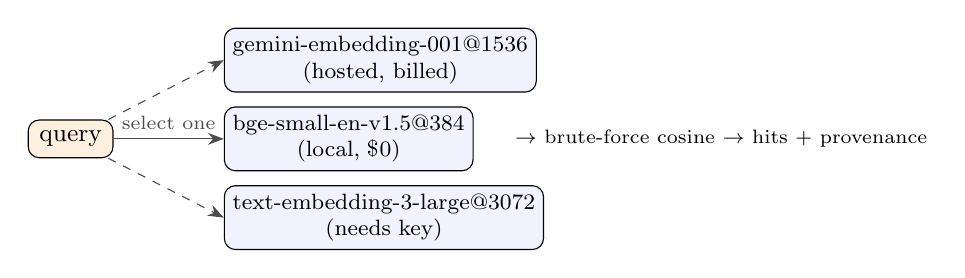
\begin{tikzpicture}[
    sp/.style={draw, rounded corners, font=\footnotesize, align=center, inner sep=3pt, fill=blue!5},
    q/.style={draw, rounded corners, font=\small, fill=orange!12, inner sep=4pt},
    arr/.style={-{Stealth[length=2mm]}, gray!60!black}]
  \node[q] (query) {query};
  \node[sp, right=14mm of query, yshift=10mm]  (a) {gemini-embedding-001@1536\\ (hosted, billed)};
  \node[sp, right=14mm of query]               (b) {bge-small-en-v1.5@384\\ (local, \$0)};
  \node[sp, right=14mm of query, yshift=-10mm] (c) {text-embedding-3-large@3072\\ (needs key)};
  \draw[arr] (query) -- node[above, font=\scriptsize, sloped]{select one} (b.west);
  \draw[arr, dashed] (query) -- (a.west);
  \draw[arr, dashed] (query) -- (c.west);
  \node[font=\scriptsize, right=4mm of b] {$\rightarrow$ brute-force cosine $\rightarrow$ hits + provenance};
\end{tikzpicture}
\caption{The vector store keeps one partition per \emph{space}. The query picks a space (a variable);
the others sit ready for an A/B without a rebuild.}
\end{figure}

\FloatBarrier
%==============================================================================
\section{Always-on cost logging}\label{sec:cost}
%==============================================================================

There is exactly \textbf{one funnel} for spend, and the rule is absolute: \emph{no module ever calls a
provider directly.} Every adapter call ends with \code{costlog.log(...)}, which appends a timestamped
row to \code{costs/usage.csv}. If \code{usd} is omitted it is \emph{estimated} from the price tables in
\code{config.py}.

Two consequences fall out of this single design choice:

\begin{enumerate}[leftmargin=1.6em, itemsep=2pt]
  \item \textbf{The ledger is complete by construction.} The only path to a provider runs through an
        adapter, and every adapter logs --- so there is no way to spend money invisibly.
        \code{costlog.summary()} aggregates the CSV by model into the running \$ total.
  \item \textbf{The free path is genuinely free.} Local embeddings (\code{fastembed}), BM25, and the
        local cross-encoder reranker all log with \code{usd=0.0}. You can develop and run the whole
        \emph{retrieval} side end-to-end without spending a cent; only hosted-model calls are billable,
        and they land in the same ledger.
\end{enumerate}

\begin{figure}[h]
\centering
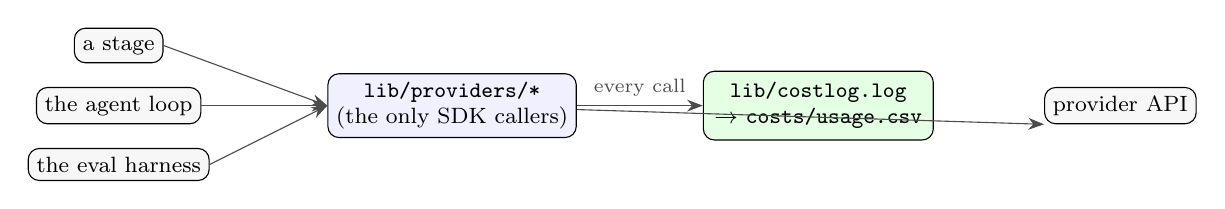
\begin{tikzpicture}[
    s/.style={draw, rounded corners, font=\footnotesize, fill=gray!6, inner sep=3pt, align=center},
    ad/.style={draw, rounded corners, font=\footnotesize, fill=blue!6, inner sep=3pt, align=center},
    log/.style={draw, rounded corners, font=\footnotesize, fill=green!10, inner sep=4pt, align=center},
    arr/.style={-{Stealth[length=2mm]}, gray!60!black}]
  \node[s] (st1) {a stage};
  \node[s, below=3mm of st1] (st2) {the agent loop};
  \node[s, below=3mm of st2] (st3) {the eval harness};
  \node[ad, right=16mm of st2] (ad) {\code{lib/providers/*}\\ (the only SDK callers)};
  \node[log, right=16mm of ad] (log) {\code{lib/costlog.log}\\ $\rightarrow$ \code{costs/usage.csv}};
  \node[s, right=14mm of log] (prov) {provider API};
  \foreach \n in {st1,st2,st3} \draw[arr] (\n.east) -- (ad.west);
  \draw[arr] (ad) -- (prov.south west);
  \draw[arr] (ad) -- node[above, font=\scriptsize]{every call} (log);
\end{tikzpicture}
\caption{Every caller routes through an adapter; every adapter logs. The cost ledger cannot have a
hole, and \$0 local calls are logged the same way as billed ones.}
\end{figure}

The adapters also \textbf{self-throttle}: bulk loops are wrapped in \code{tenacity} retry-with-backoff
that treats \code{429 / RESOURCE\_EXHAUSTED / 503 / 5xx} as transient and waits-and-retries
exponentially. A long run bends to the provider's rate limit instead of crashing partway --- the same
lesson the OCR step learned. (For true bulk, the plan is the Gemini Batch API: $-50\%$, no per-minute
cap; gated until David says go.)

\FloatBarrier
%==============================================================================
\section{Provenance and archival standards}\label{sec:prov}
%==============================================================================

An archive's whole value is \emph{trust}: a claim you can't trace is worthless to a historian. So
provenance is threaded through every layer.

\begin{itemize}[leftmargin=1.4em, itemsep=2pt]
  \item \textbf{Chunks} carry \code{\{doc\_id, rid, page, pdf\_page, \dots\}} from the moment they're
        built.
  \item \textbf{The vector store} keeps that metadata beside every vector, so a hit already knows
        where it came from.
  \item \textbf{The knowledge graph} attaches source \code{rid}s to every node and edge --- so even an
        \emph{inferred} fact points back at the regions that justify it.
  \item \textbf{Answers} cite \code{doc\_id + rid + page (+ vertices)}; the app's citation modal turns
        those vertices into a \textbf{deep-zoom box on the page image} (IIIF Presentation 3.0
        manifests + Web Annotations) and offers the source PDF to download.
\end{itemize}

On the standards side: the graph aligns to \textbf{RiC-O} (ICA Records in Contexts, proven on
scholarly correspondence) and exports RDF/JSON-LD; dates use \textbf{EDTF} (the Library of Congress
standard for uncertain/approximate/partial dates --- exactly the ``c.\ 1929'' /
``Mar.\ 30''-with-no-year mess this corpus is full of); entities are reconciled to \textbf{Wikidata /
VIAF / GeoNames / Getty~TGN} for global IDs; observability rides on \textbf{OpenTelemetry / Phoenix}.

\FloatBarrier
%==============================================================================
\section{The tiers (and the stages that fill them)}\label{sec:tiers}
%==============================================================================

The build is organised into additive tiers (from \code{RESEARCH\_PLAN.md}). Each raises the ceiling,
and each new capability becomes a \emph{toggleable tool} in the dev app --- so you can measure exactly
what each one buys you.

\begin{figure}[h]
\centering
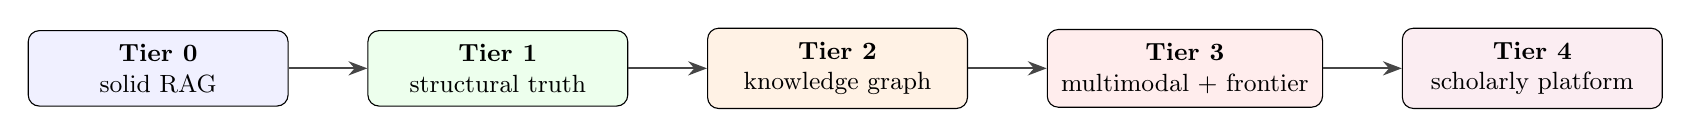
\begin{tikzpicture}[
    t/.style={draw, rounded corners, font=\small, align=center, inner sep=5pt, minimum width=33mm},
    arr/.style={-{Stealth[length=2.4mm]}, gray!55!black, thick}]
  \node[t, fill=blue!6]   (t0) {\textbf{Tier 0}\\ solid RAG};
  \node[t, fill=green!7, right=10mm of t0]  (t1) {\textbf{Tier 1}\\ structural truth};
  \node[t, fill=orange!10, right=10mm of t1] (t2) {\textbf{Tier 2}\\ knowledge graph};
  \node[t, fill=red!7, right=10mm of t2]    (t3) {\textbf{Tier 3}\\ multimodal + frontier};
  \node[t, fill=purple!7, right=10mm of t3] (t4) {\textbf{Tier 4}\\ scholarly platform};
  \draw[arr] (t0) -- (t1); \draw[arr] (t1) -- (t2);
  \draw[arr] (t2) -- (t3); \draw[arr] (t3) -- (t4);
\end{tikzpicture}
\caption{The recommended path. Each tier is additive; eval gates each step.}
\end{figure}

\begin{description}[leftmargin=0pt, itemsep=4pt]
  \item[Tier 0 --- solid RAG.] \stage{embed\_corpus} $\rightarrow$ the vector store $\rightarrow$
        \code{lib/retrieval.py} (router $\rightarrow$ query transforms like HyDE $\rightarrow$ hybrid
        BM25 + dense fused with RRF $\rightarrow$ cross-encoder rerank $\rightarrow$ optional
        Self-RAG/CRAG grading) $\rightarrow$ cited generation. This alone is a strong archival
        search/QA tool.
  \item[Tier 1 --- structural truth.] The corpus problems, built first because everything downstream
        depends on getting the \emph{units} right:
        \begin{itemize}[leftmargin=1.2em, itemsep=1pt]
          \item \stage{stitch\_notebooks} (A1) --- reconstruct \emph{logical} entries across
                ``Page N Cont.'' breaks, so a favour split over two pages is retrieved (and cited) as
                one whole thought.
          \item \stage{normalize\_dates} (A2) --- combine the entry's month/day with the \emph{page's}
                archival year, carry forward the last-seen date, capture \emph{bitemporal}
                enrolled-vs-reported pairs $\rightarrow$ EDTF. Free rule path; gated LLM normaliser.
          \item \stage{contextualize\_chunks} --- Anthropic-style \emph{Contextual Retrieval}: prepend
                a 1--2 sentence situating preamble to each chunk \emph{before} embedding/BM25, so the
                bare ``22\ \ Cured.'' entry stops being invisible. The highest-leverage retrieval
                upgrade for \emph{this} corpus.
          \item \stage{extract\_entities} (NER) --- two passes: a \emph{free} structured harvest (the
                labelled fields are entities we already know the type of), then a gated LLM pass over
                the prose for rich nested entities.
          \item \stage{resolve\_entities} (A3) --- the classic ER pipeline (normalise $\rightarrow$
                block $\rightarrow$ match $\rightarrow$ cluster $\rightarrow$ canonicalise
                $\rightarrow$ authority-reconcile) so ``Grace.'', ``Grace Panyard'', and ``Mrs.\ Grace
                Panyard'' collapse to one authority record.
        \end{itemize}
  \item[Tier 2 --- knowledge graph + GraphRAG.] \stage{build\_graph} --- a temporal property graph
        (networkx) aligned to RiC-O, exported to RDF; community detection + summaries for thematic
        questions. \stage{index\_sources} --- a SQLite \textbf{FTS5} full-text index + \textbf{IIIF}
        manifests + text-layer searchable PDFs (all free, all local).
  \item[Tier 3 --- multimodal + frontier.] \stage{colpali\_index} --- visual retrieval over the
        \emph{page images} with late interaction (catches what the OCR missed), fused with text.
        \stage{raptor} --- a recursive cluster-and-summarise tree for global/thematic questions.
  \item[Tier 4 --- scholarly platform.] IIIF deep-zoom citations, Linked-Data exports
        (RiC-O / EDTF / authority IDs), fine-tuned models (deferred per David), hosting + drift
        monitoring.
\end{description}

\begin{tcolorbox}[colback=gray!5, colframe=gray!50!black, sharp corners, boxrule=0.5pt,
                  title=\bfseries Current state]
\stage{embed\_corpus} and \stage{normalize\_dates} are wired into \code{run.py} and the base
embeddings are built (\code{gemini-embedding-001@1536} and a free local \code{bge-small-en-v1.5@384}).
The remaining stages exist as substantial drafted modules and become live as they are integrated and
tested. The DAG is fully \emph{inspectable} today (\code{python run.py graph}); paid stages stay gated
until explicitly run.
\end{tcolorbox}

\FloatBarrier
%==============================================================================
\section{Where the axes and tiers meet the user: the dev app}
%==============================================================================

The capabilities surface in a FastAPI app (\code{app/server.py}) that exposes a \textbf{tool-using
agent}: given a question plus the three model variables and a set of \emph{enabled tools}, it runs a
Gemini function-calling loop over \emph{only those tools} and returns
\code{\{answer, citations[], trace[], grade, cost\}}. Each capability is a plugin in \code{app/tools/}
(\code{vector\_search}, \code{pdf\_fulltext\_search}, \code{graph\_query}, \code{entity\_lookup},
\code{temporal\_query}, \code{community\_summary}), so it shows up as a \emph{toggle} in the UI ---
which is precisely how you measure what each tier contributes. The server never calls a provider
directly; every turn routes through \code{lib/providers/* $\rightarrow$ lib/costlog}, so the ledger
stays complete and the free path stays \$0.

The \code{eval/} harness closes the loop: a set of \textbf{golden questions} (each with
\code{ground\_truth}, \code{expected\_where}, \code{relevant\_doc\_ids}) is run through the real stack
and scored on the RAGAS/ARES metrics (faithfulness, context precision/recall, answer relevance) for
\emph{every combination} of the three axes --- so ``which config to ship'' is an empirical read-off,
not a guess.

\FloatBarrier
%==============================================================================
\section{Recommendations: how to extend}
%==============================================================================

The whole point of the architecture is that extension is \emph{local}. The four common moves:

\begin{itemize}[leftmargin=1.4em, itemsep=2pt]
  \item \textbf{Add a stage.} Write a function in \code{stages/}, then register a
        \code{Stage(name, fn, deps, inputs, outputs)} in \code{run.py}. The DAG handles staleness and
        ordering --- you never write scheduling code.
  \item \textbf{Add an embedding space.} Add a \code{(model, dim)} tuple to
        \code{config.EMBEDDING\_MATRIX} (and the model to \code{config.EMBEDDINGS} if new). The embed
        stage re-embeds \emph{only the new space}.
  \item \textbf{Add a model.} Add it to \code{config.LLMS / EMBEDDINGS / RERANKERS} with its price,
        and add the one provider branch in the matching adapter. Stages reading \code{DEFAULTS} pick
        it up with no edits.
  \item \textbf{Add an agent tool.} Drop a module in \code{app/tools/}; it appears as a toggle in the
        UI and a function declaration to the LLM.
\end{itemize}

\begin{tcolorbox}[colback=blue!4, colframe=blue!50!black, sharp corners, boxrule=0.5pt]
\textbf{Rule of thumb:} if you find yourself editing a \emph{stage} to swap a model, stop --- that's a
sign the variable belongs in \code{config.py} instead.
\end{tcolorbox}

%==============================================================================
\section{Caveats}
%==============================================================================

\begin{caveatbox}[Read before you run anything billed]
\begin{itemize}[leftmargin=1.2em, itemsep=2pt]
  \item \textbf{Prices in \code{config.py} are placeholders.} They let \code{costlog} \emph{estimate}
        spend; verify each against the provider's current pricing page before any billed run. Nothing
        is billed until a stage is actually executed.
  \item \textbf{Several stages are drafted, not yet live.} The DAG is inspectable now; integration +
        small smoke-tests gate each paid stage. \code{NotImplementedError} is the honest placeholder.
  \item \textbf{Fingerprints hash \emph{file contents}, not semantics.} A whitespace-only edit to a
        stage's source \emph{will} mark it stale (it changes \code{inspect.getsource}). That is the
        conservative, correct default --- better to re-run than to silently serve a stale artifact.
  \item \textbf{The vector store is brute-force cosine.} Instant at $\sim$9k vectors, deliberately so;
        swappable for LanceDB/FAISS later \emph{without changing callers} if the corpus grows.
  \item \textbf{Heavy/paid steps are deliberately deferred.} ColPali (vision model + GPU) is
        scaffolded but its heavy index build is flagged; full LLM NER and full multi-space embedding
        run only after a small cost-scoping batch, and only when David says go.
\end{itemize}
\end{caveatbox}

%==============================================================================
\section{Sources}
%==============================================================================

\paragraph{In-repo.} \code{README.md} (design commitments + milestones); \code{RESEARCH\_PLAN.md}
(techniques, tiers, research basis); \code{config.py} (the three axes + prices);
\code{lib/pipeline.py} (the DAG engine); \code{lib/costlog.py} (the cost funnel);
\code{lib/chunks.py} / \code{lib/vectorstore.py} (data shapes + the partitioned store);
\code{lib/providers/\{llm,embed,rerank\}.py} (the adapters); the \code{stages/} modules and the
\code{app/} server + tools.

\paragraph{External (from \code{RESEARCH\_PLAN.md}).} Anthropic Contextual Retrieval; RiC-O (ICA
Records in Contexts); EDTF (Library of Congress / ISO~8601-2); Splink (probabilistic record linkage);
RAPTOR (Sarthi et al.\ 2024); ColPali (late-interaction visual retrieval); RAGAS / ARES (RAG
evaluation); OpenTelemetry / Arize Phoenix (observability).

\end{document}
